\documentclass[12pt,onecolumn,notitlepage]{article}
\usepackage[margin=0.5in]{geometry}
\usepackage{amsmath}
\usepackage{gensymb}
\usepackage{graphicx}
\usepackage{amsthm}
\usepackage{mathrsfs}
\usepackage{txfonts}
\usepackage{cite}
\usepackage{cases}
\usepackage{subfig}
\usepackage[breaklinks=true]{hyperref}
\usepackage{listings}
\usepackage[latin1]{inputenc}
\usepackage{color}
\usepackage{array}
\usepackage{longtable}
\usepackage{calc}
\usepackage{multirow}
\usepackage{hhline}
\usepackage{ifthen}
\usepackage{amssymb}

\providecommand{\pr}[1]{\ensuremath{\Pr\left(#1\right)}}
\providecommand{\sbrak}[1]{\ensuremath{{}\left[#1\right]}}
\providecommand{\lsbrak}[1]{\ensuremath{{}\left[#1\right.}}
\providecommand{\rsbrak}[1]{\ensuremath{{}\left.#1\right]}}
\providecommand{\brak}[1]{\ensuremath{\left(#1\right)}}
\providecommand{\lbrak}[1]{\ensuremath{\left(#1\right.}}
\providecommand{\rbrak}[1]{\ensuremath{\left.#1\right)}}
\providecommand{\cbrak}[1]{\ensuremath{\left\{#1\right\}}}
\providecommand{\lcbrak}[1]{\ensuremath{\left\{#1\right.}}
\providecommand{\rcbrak}[1]{\ensuremath{\left.#1\right\}}}
\newcommand*{\comb}[2]{{}^{#1}C_{#2}}
\title{Hardware Assignment Report}
\author{Pallala Rishitha (BT22BTECH11011)}
\date{}
\begin{document}
\maketitle
\textbf{\LARGE{Assignment :}}\\\\
Random Number generation using Shift Registers.\\\\


   \section*{Components required :}
\begin{enumerate}

  \setlength\itemsep{0pt} % Adjust the spacing between points
  \item     555 IC (Timer IC)-1
\item D flip-flops(7474)-2
\item XOR gate(7486) -1
\item Resistor(1M$\Omega$)-1
\item Resistor(1K$\Omega$)-1
\item Capacitor(100nF)-1
\item Capacitor(10nF)-1
\item Connecting wires-20
\item Breadboard -1
\item Seven-segment display(common anode)-1
\item decoder(7447)-1

\end{enumerate} 
   \section*{Function of each Component:}
\begin{enumerate}
  \setlength\itemsep{0pt}
  \item     Breadboard: It provides a platform for connecting and prototyping electronic components without the need for soldering.

   \item Decoder: It decodes the binary inputs from the D-flip flops and activates the corresponding outputs based on the binary pattern.

   \item  D-flip flops: They are sequential logic circuits that store and transfer binary data, In this context, they act as part of the shift register, holding the binary values and shifting them based on the clock pulses.

    \item Resistors: They are passive electronic components that control the flow of electric current in a circuit, In this context, resistors may be used to provide current limiting or voltage division.

    \item Capacitors: They are passive components used to store and release electrical energy,In this circuit, capacitors may be used in conjunction with resistors to determine the frequency of the clock signal produced by the 555 IC.

    \item Connecting wires: These are used to establish electrical connections between different components on the breadboard.

   \item  Seven-segment display: It is a display device that can show numerical digits and certain characters, In this circuit, it is used to display the generated random numbers.

   \item  XOR gate: It is a logic gate that outputs true (1) if the number of input signals that are true (1) is odd, In the context of the shift register, XOR gates introduce feedback loops that create the randomness in the system.

    \item 555 IC: It is a popular integrated circuit that can be configured as an astable multivibrator, producing a continuous stream of clock pulses, In this circuit, the 555 IC is used to generate the clock signal for the shift register.
\end{enumerate} 

\begin{figure}[h!]
  \centering
  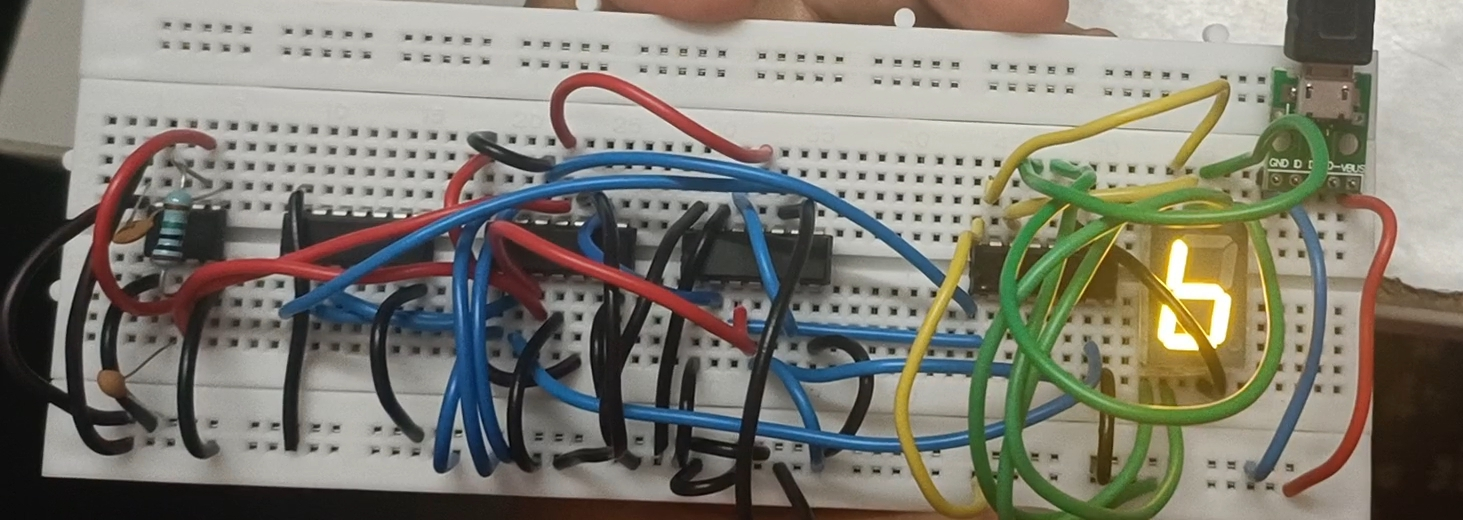
\includegraphics[width=0.5\textwidth]{circuit.jpg}
  \caption{Random Number generation using Shift registers and XOR Gate}
  \label{fig:Circuit}
\end{figure}
\begin{figure}[h!]
  \centering
  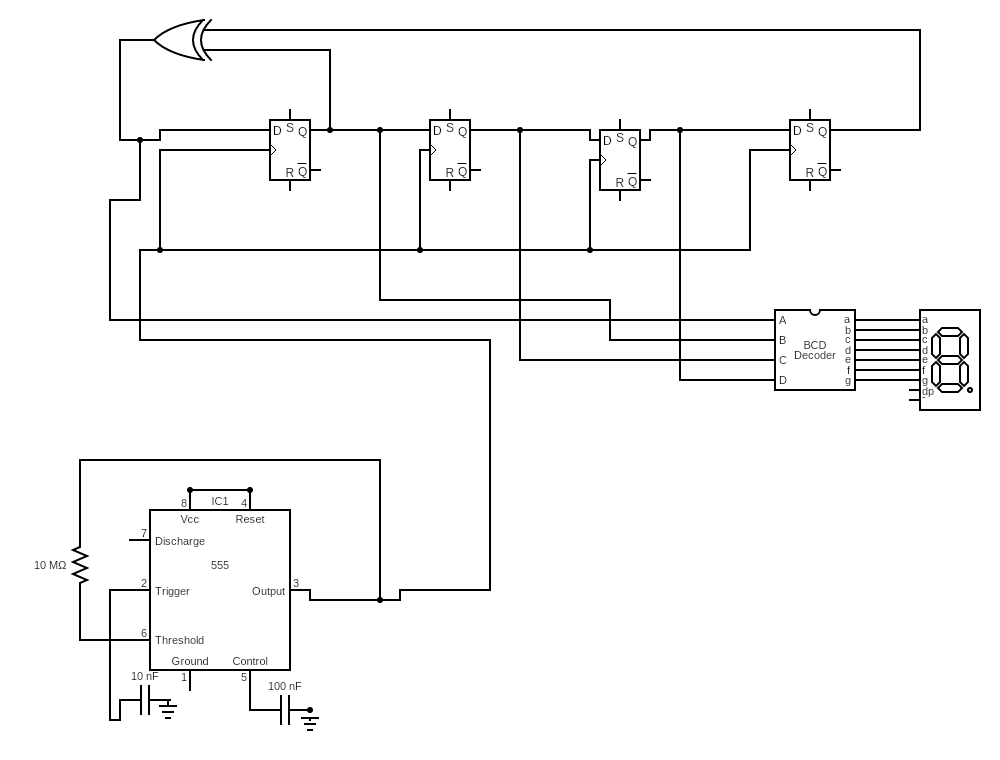
\includegraphics[width=0.5\textwidth]{blockdiagram.png}
  \caption{Block Diagram of the circuit}
  \label{fig:Block Diagram}
\end{figure}

 

 


\end{document}
